% !TEX root = ../main.tex

\section{Plateforme matérielle}
\label{section:plateforme_materielle}

    Dans cette section, nous allons détailler la carte que nous avons utilisée pour effectuer nos travaux en portant une attention particulière sur la hiérarchie mémoire.

    % Ressources en ligne :
    %
    % i.MX6 DDR3 RAM-Performance 32 bit vs. 64 bit interface.
    %     https://community.nxp.com/thread/329671
    %
    % i.MX6 - question about DDR memory bandwidth utilization
    %     https://community.nxp.com/thread/320997
    %
    % https://community.arm.com/thread/8295
    %     https://community.arm.com/thread/8295
    %
    % What is AXi?
    %     https://www.youtube.com/watch?v=0Dt8rWJdiJo
    %
    % Migrating from AHB to AXI based SoC Designs
    %     https://www.doulos.com/knowhow/arm/Migrating_from_AHB_to_AXI/
    %
    % Introduction to AXI
    %     http://www.analyticsengines.com/developer-blog/introduction-to-axi/
    %
    % Why is the I-cache designed as VIPT, while the D-cache as PIPT?
    %     https://community.arm.com/thread/5874
    %
    % Line Fill Buffers
    %     https://docs.google.com/presentation/d/1b-woFnas1HL5e4nkbyFAPjTrd884pBG98etEEjqSO_o/edit#slide=id.g20269671_3_105

%     \itodo{
%         Attributs du cache :
%         \begin{itemize}
%             \item Taille d'une ligne de cache
%             \item Taille d'un mot mémoire
%             \item Cache associatif : niveaux d'associativité
%             \item Politique de remplacement des données
%             \item Politique d'écriture utilisée
%             \item Politique d'allocation utilisée
%             \item Indexation du cache : avantages et inconvénients
%             \item Tampons utilisés
%         \end{itemize}
%   }

    Nous utilisons une carte i.MX6Q Sabre Lite comme plateforme matérielle de référence pour nos travaux.
    Ce choix est motivé par plusieurs raisons.
    Tout d'abord, nos travaux s'inscrivant dans le cadre d'une thèse CIFRE, le matériel choisi se devait d'être représentatif de celui utilisé dans l'industrie.
    C'est le cas de cette carte, initialement conçue pour des applications multimédias.
    Une variante automobile~\cite{manuel:i_MX_6Dual_6Quad_automotive_and_infotainment_applications_processors} de cette carte a d'ailleurs été largement utilisée par un grand nombre de fabricants et de fournisseurs de l'industrie automobile.
    La deuxième raison qui motive notre choix est que cette carte offre un bon niveau de documentation.

    % Nos travaux s'inscrivant dans le cadre d'une thèse CIFRE, le matériel de référence que nous utilisons se devait d'être représentatif de celui utilisés en contexte industriel.
    % Notre choix s'est porté sur la carte embarqué i.MX6 SABRE Lite~\cite{sabrelite}.
    % Il s'agit d'une carte de développement à bas coût, initialement prévue pour exécuter des applications multimédia en utilisant les systèmes d'exploitation Linux et Android.
    % Notons qu’il existe une variante automobile de cette plate-forme (SABRE Automotive \cite{manuel:i_MX_6Dual_6Quad_automotive_and_infotainment_applications_processors}) qui a largement été utilisée par un grand nombre de fabricants et de fournisseurs du monde automobile.

    \begin{figure}[!ht]
        \centering
        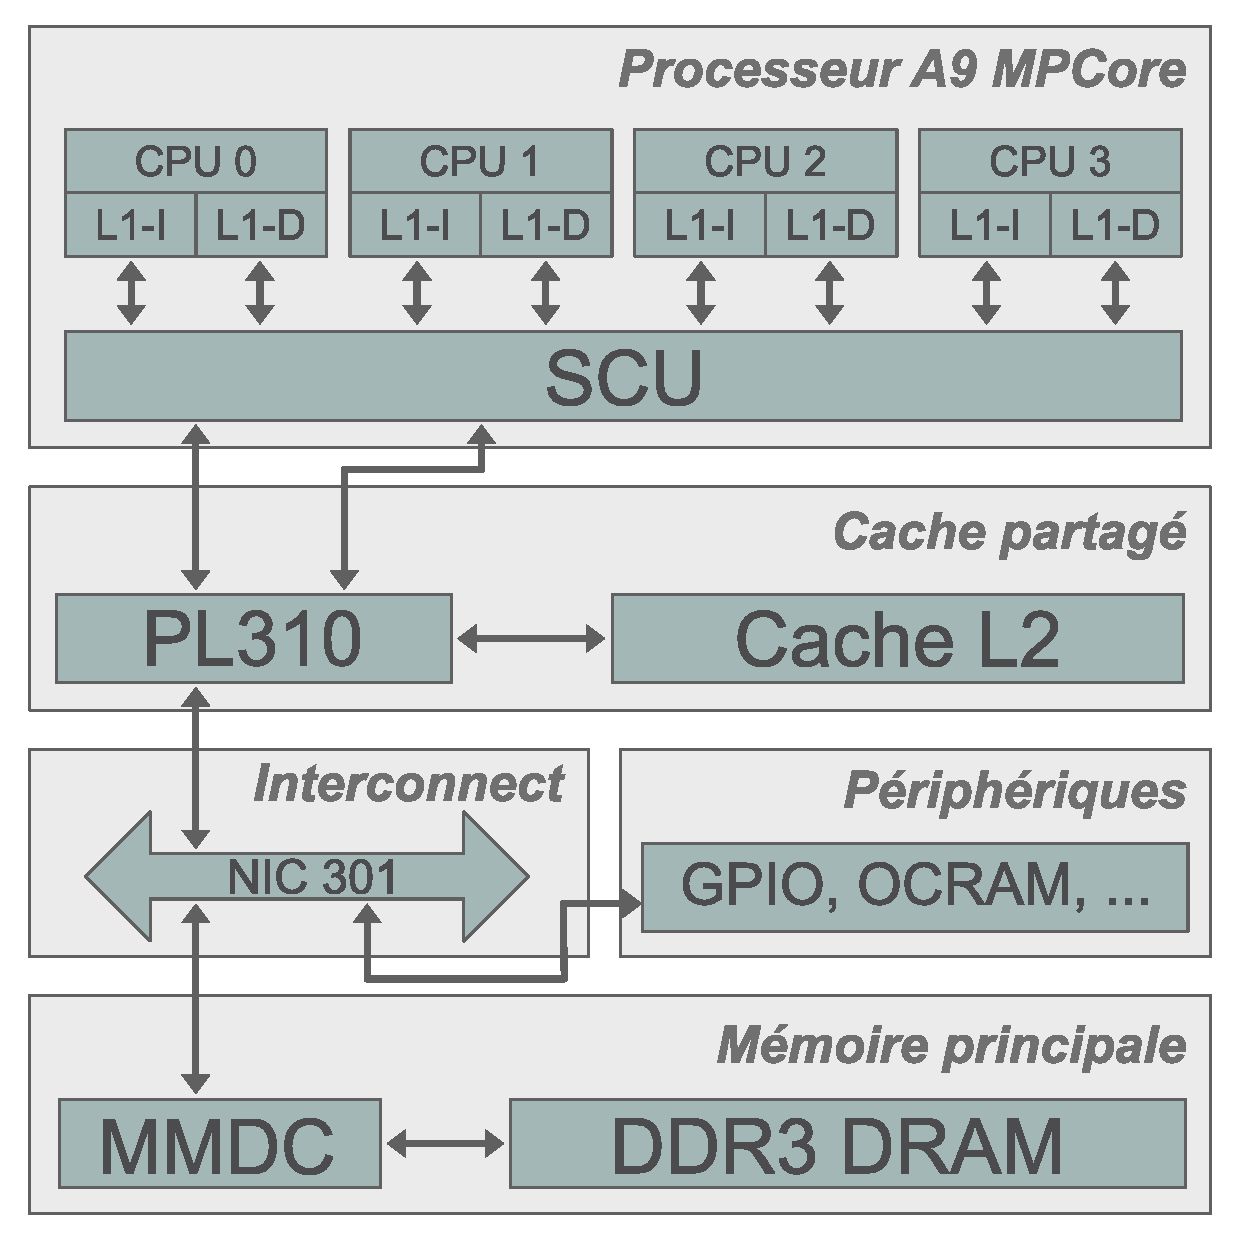
\includegraphics[width=0.5\linewidth]{sabrelite-block-diagram}
        \caption{Architecture matérielle simplifiée de la carte SABRE Lite}
        \label{fig:archiIMX6}
    \end{figure}

    L'unité de calcul de la carte est composée d'un processeur \emph{i.MX 6}, basé sur un quatre-cœurs \emph{Cortex A9 MPCore}, connecté à un cache L2 externe \emph{PL310} d'un mégaoctet. Le contrôleur mémoire \emph{MMDC} qui gère l'accès à un gibioctet de mémoire DDR3 est connecté à un bus d'interconnexion \emph{NIC-301} qui assure la connexion entre les consommateurs de mémoire (Processeur, GPU …) et différents périphériques (PCIe, MMDC, OCRAM, ...).

    L'ensemble des composants sont reliés par des bus \emph{AXI} (\emph{AMBA eXtensible Interface}) un standard développé par ARM qui effectue une liaison point à point pour relier deux modules matériels. Un module maître amorce une transaction de données en lecture ou en écriture vers un module esclave qui reçoit et répond à la transaction. L'ensemble de ces bus est équipé de deux canaux séparés qui permettent de traiter les transactions en lecture en parallèle de celles en écriture.
    %http://www.design-reuse.com/articles/24123/amba-ahb-to-axi-bus-comparison.html)

    %La figure \ref{fig:archiIMX6} affiche une vue d'ensemble simplifiée de la plate-forme i.MX 6 SABRE Lite.

    Nous allons maintenant, nous appuyer sur la vue d'ensemble de l'architecture de notre plateforme, présentée dans la figure \ref{fig:archiIMX6}, pour détailler plus précisément les composants matériels utilisés dans nos travaux. Nous allons, dans une première partie, effectuer une description du processeur implanté au sein de notre carte pour ensuite, dans les parties suivantes, étudier les différents niveaux de hiérarchie mémoire, matérialisés par les caches L1, le cache L2 et le contrôleur mémoire, qui sont partagés entre les cœurs et les périphériques matériels.

%    \FloatBarrier

    %\subsection{Processeur cortex-A9 MPCore}
    \subsection{Processeur}

        Le processeur de notre carte est composé de quatre cœurs \emph{cortex-A9} regroupés ensemble au sein d'un unique circuit intégré intitulé \emph{Cortex-A9 MPCore}.

        \subsubsection{Cœur cortex-A9}

            % === 12.3 Platform configuration ===
            %
            % --- Cortex-A9 Core configuration ---
            %
            %     DCACHESIZE              32      L1 Data cache size
            %     ICACHESIZE              32      L1 Instruction cache size
            %     TLBSIZE                 128     JAZELLE_PRESENT Yes Providing ARM's Jazelle technology hardware extensions.
            %     FPU_PRESENT             No      The FPU functions are provided by NEON, thus additional FPU cannot be used.
            %     NEON_PRESENT            Yes     Use MPE, NEON Co-Processor and FPU
            %     PRELOAD_ENGINE_PRESENT  No      May only be beneficial in Video processing.
            %
            %     Chapter 1 Introduction
            %     1.1 About the Cortex-A9 processor
            %
            % The Cortex-A9 processor is a high-performance, low-power, ARM macrocell with an L1 cache subsystem that provides full virtual memory capabilities. The Cortex-A9 processor implements the ARMv7-A architecture and runs 32-bit ARM instructions, 16-bit and 32-bit Thumb instructions, and 8-bit Java bytecodes in Jazelle state.
            %
            % 1.5 Interfaces
            %     The processor has the following external interfaces:
            %         AMBA AXI interfaces
            %         Debug v7 compliant interface, including a debug APBv3 external debug interface
            %         DFT.
            %     For more information on these interfaces see:
            %         AMBA AXI Protocol Specification
            %         CoreSight Architecture Specification
            %         Cortex-A9 MBIST Controller Technical Reference Manual
            %
            % Chapter 2 Functional Description
            %     2.2 Interfaces
            %     2.4 Power management
            %
            % Chapter 7 Level 1 Memory System
            %
            % Chapter 11 Performance Monitoring Unit

            L'unité de calcul \emph{Cortex-A9}, présentée dans la figure \ref{fig:cortex_A9_uniprocessor_system}, est un processeur à haute performance et à faible consommation conçu par la société ARM suivant l'architecture \emph{ARMv7-A} \cite{manuel:ARMv7} et les jeux d'instructions 32-bit ARM, 16-bit et 32-bit Thumb \cite{manuel:cortex_A9_technical_reference_manual}.

            \begin{figure}[!ht]
                \centering
                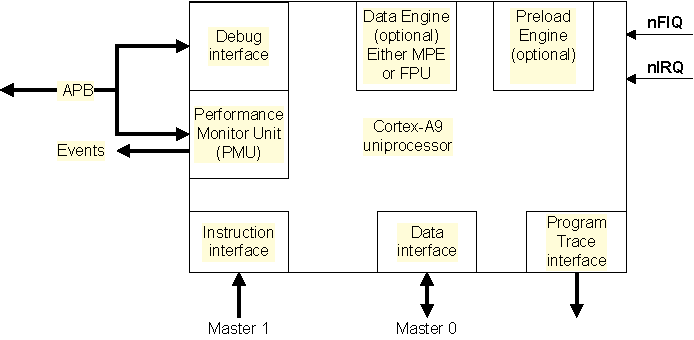
\includegraphics[width=0.9\linewidth]{cortex_A9_uniprocessor_system}
                \caption{Système monoprocesseur Cortex-A9 \cite{manuel:cortex_A9_technical_reference_manual}}
                \label{fig:cortex_A9_uniprocessor_system}
            \end{figure}

            Chaque processeur possède une unité de mesure des performances (\emph{Performance Monitoring Unit}) qui contient sept compteurs matériels pouvant être utilisés aussi bien pour récupérer des statistiques sur les opérations exécutées par le processeur (Nombre de cycles …) que sur les accès réalisés par le système mémoire (Cache L1 MISS, Cache L1 HIT, ...). Un des compteurs est configuré en dur pour compter le nombre de cycles effectués par le processeur tandis que les six compteurs restants peuvent être configurés pour enregistrer un des 58 événements mesurables.
            Nous utiliserons ces compteurs pour caractériser en partie le comportement des applications.



        \subsubsection{Processeur cortex-A9 MPCore}

            % Chapter 12 ARM Cortex A9 MPCore Platform (ARM)
            %
            % 12.3.1 Platform and SCU configuration \cite{i.MX_6Dual_6_Quad_Applications_Processor_Reference_Manual}
            % Table 12-3. Cortex-A9 configuration
            %
            % Option                  Selected    Value Comments
            % MP_MODE                 Yes         Multi-Processor mode
            % POWER_DOMAIN_WRAPPER    No          Wrappers to support power off of individual cores.
            % PTM_INTERFACE_PRESENT   Yes         Use PTM as part of Trace/Debug logic.
            % PARITY                  Yes         Using RAM arrays which support parity.
            % CORE_NUM                2/4         1 Number of cores
            % INT_NUM                 128         Number of interrupts (SPIs) in GIC
            % ACP_PRESENT             No          Accelerator Coherency Port (ACP)
            % MASTER_NUM              2           Number of 64-bit AXI output master ports.

            Le processeur Cortex-A9 MPCore, présenté dans la figure \ref{fig:example_multiprocessor_configuration}, est constitué d'un ensemble de quatre processeurs Cortex A9 regroupés et connectés à une unité de contrôle nommée \emph{Snoop Control unit}.

            \begin{figure}[!ht]
                \centering
                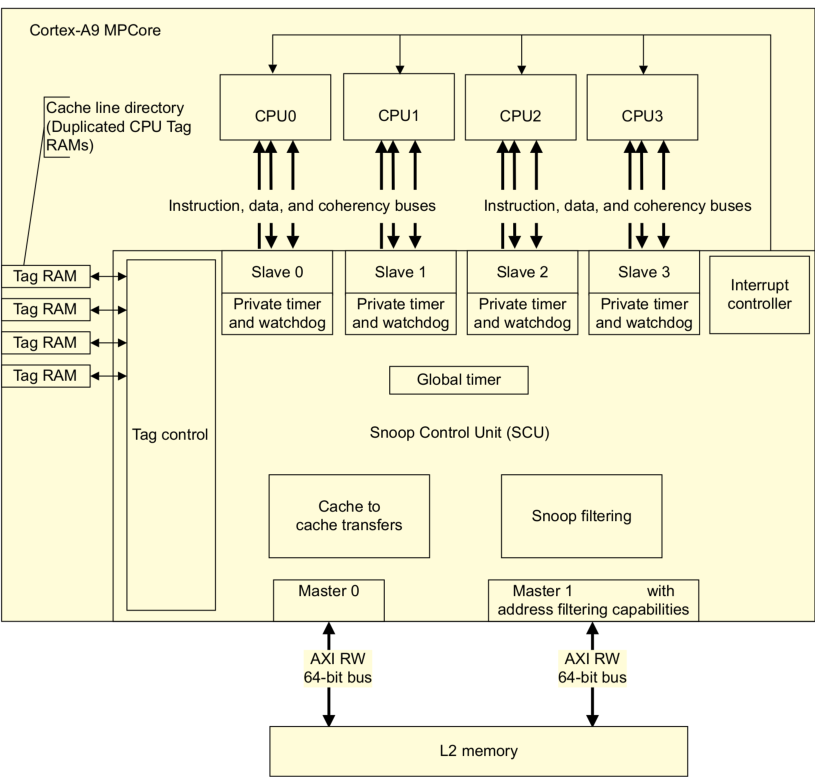
\includegraphics[width=\linewidth]{example_multiprocessor_configuration_2}
                 \caption{Exemple de configuration multiprocesseur \cite{manuel:cortex_a9_mpcore_trm}}
                 \label{fig:example_multiprocessor_configuration}
             \end{figure}
% 
            La SCU maintient la cohérence entre les caches des différents processeurs du groupe en utilisant un protocole dérivé de \emph{MESI}. Elle arbitre également les requêtes émises par les processeurs vers les niveaux de hiérarchie mémoire supérieurs et génère les accès mémoire correspondants.

            Le processeur Cortex-A9 MPCore contient un ensemble de périphériques mappés en mémoire incluant un temporisateur global, ainsi qu'un \emph{watchdog} et un temporisateur privé pour chacun des processeurs du groupe.
            %
            Un contrôleur d'interruptions respectant l'architecture \emph{Generic Interrupt Controller} \cite{manuel:gic} est également présent. Localisé, au sein du processeur MPCore, il a pour rôle de centraliser toutes les sources d'interruptions avant de les répartir vers les processeurs individuels.

            Le processeur Cortex-A9 MPCore est connecté à un contrôleur de cache externe de type PL310 de niveau 2 par deux bus AXI 64 bits et peut, théoriquement, générer (\emph{maître}) jusqu'à 24 transactions par processeur vers le cache L2 (\emph{esclave}).
            % Cortex A* MPCORe AXI issuing capabilities
            % http://infocenter.arm.com/help/index.jsp?topic=/com.arm.doc.dui0305c/Cbaifdib.html
            %
            % L2 Prefetch Hint feature}
            %\optionnel{Pour augmenter les performances du système le cœur est doté d'une unité désactivable de préchargement qui détecte les patterns de chargement mémoire réguliers et envoie des requêtes au contrôleur PL310 pour précharger des lignes de mémoire dans le cache L2.}

            % Manuel Cortex-A9 TRM
            %
            % Prefetch hint to the L2 memory interface
            %
            % The Cortex-A9 processor can generate prefetch hint requests to the L2 memory controller. The prefetch hint requests are non-compliant AXI read requests generated by the Cortex-A9 processor that do not expect any data return.
            %
            % You can generate prefetch hint requests to the L2 by:
            % •   Enabling the L2 Prefetch Hint feature, bit [1] in the ACTLR. When enabled, this feature enables the Cortex-A9 processor to automatically issue L2 prefetch hint requests when it detects regular fetch patterns on a coherent memory. This feature is only triggered in a Cortex-A9 MPCore processor, and not in a uniprocessor.

            % Manuel L2C-310 TRM
            %
            % Prefetch hints
            %
            % When you configure the Cortex-A9 processor to run in SMP mode, the automatic data prefetchers, implemented in one or more CPUs, issues special read accesses to the L2C-310. See the Cortex-A9 TRM. These special reads are called Prefetch Hints. They are indicated when a device sets ARUSERSx[8] to 1. When the L2C-310 slave ports receive such prefetch hints, they do not send any data back to the Cortex-A9 processor, they allocate the targeted cache line into the L2 cache for a miss. This behavior is not compatible with AXI. When a master other than a Cortex-A9 processor drives the L2C-310 ARUSERSx[8] must be tied 0.

            % Partie 22.1 Cache coherency du cortex a series programmers guide
            % The coherency management is implemented using a MESI-based protocol,

            % MPcore manuel
            % When Address Filtering is enabled, SCU Control Register bit [1] = 1, any access that fits in the address range between the Filtering Start Address and the Filtering End Address is issued on the AXI Master port M1. All other accesses outside of this range are directed onto AXI Master port M0.This filtering rule is applied independently of the AXI request type and attributes. When Address Filtering is disabled, accesses can be issued indifferently on AXI Master port M0 or AXI Master port M1, provided that the AXI ordering rules are respected. However, in this case, locked and exclusive accesses are always issued on AXI Master port M0.

            %The Cortex-A9 MPCore processor consists of:
            %    • From one to four Cortex-A9 processors in a cluster and a Snoop Control Unit (SCU) that can be used to ensure coherency within the cluster.
            %    • A set of private memory-mapped peripherals, including a global timer, and a watchdog and private timer for each Cortex-A9 processor present in the cluster.
            %    • An integrated Interrupt Controller that is an implementation of the Generic Interrupt Controller architecture. The integrated Interrupt Controller registers are in the private memory region of the Cortex-A9 MPCore processor

            % The Interrupt Controller is a single functional unit that is located in a Cortex-A9 MPCore design. It is responsible for centralizing all interrupt sources before dispatching them to each individual Cortex-A9 processor. There is one interrupt interface per Cortex-A9 processor.

            % The Cortex-A9 MPCore L2 interface can have two 64-bit wide AXI bus masters. In a two bus master configuration there is also an option to configure address filtering.

            % Individual Cortex-A9 processors in the Cortex-A9 MPCore cluster can be implemented with their own hardware configurations.

            % The SCU connects one to four Cortex-A9 processors to the memory system through the AXI interfaces.
            % The SCU functions are to:
            %     • maintain data cache coherency between the Cortex-A9 processors
            %     • initiate L2 AXI memory accesses
            %     • arbitrate between Cortex-A9 processors requesting L2 accesses
            %     • manage ACP accesses.
            %
            % The Cortex-A9 MPCore processor consists of:
            %     • From one to four Cortex-A9 processors in a cluster and a Snoop Control Unit (SCU) that can be used to ensure coherency within the cluster.
            %     • A set of private memory-mapped peripherals, including a global timer, and a watchdog and private timer for each Cortex-A9 processor present in the cluster.
            %     • An integrated Interrupt Controller that is an implementation of the Generic Interrupt Controller architecture. The integrated Interrupt Controller registers are in the private memory region of the Cortex-A9 MPCore processor.
            %
            %
            % Snoop Control Unit (SCU), that maintains L1 data cache coherency.

        \subsubsection{Impact sur les interférences}
        \label{processeur:impacts_sur_nos_travaux}
        Bien que les cœurs Cortex-A9 sont indépendants les uns des autres, un couplage existe au travers de l'interface MPCore, et plus particulièrement la \emph{SCU}. 
        Celle-ci a deux fonctions: maintenir la cohérence des données entre les caches L1 des différents cœurs et arbitrer l'accès au cache L2.
        % Ces fonctions sont toutes les deux sources d'interférence entre les coeurs.

        Le maintien de la cohérence entre les cœurs entraîne une augmentation du nombre d'invalidations lorsque des données sont partagées.
        Il s'agit d'une forme d'interférence spatiale qui est propre aux applications utilisant le modèle SMP.
        Vu que nos travaux se concentrent sur le modèle AMP, nous ne tiendrons pas compte de ce type d'interférence.
 
        En outre, la \emph{SCU} a également pour vocation d'arbitrer les différentes requêtes émises par les cœurs vers la hiérarchie mémoire de niveau supérieur. Or, la capacité du cache à répondre en parallèle aux requêtes d'accès étant limitée, l'ordre d'émission des requêtes vers la hiérarchie mémoire de niveau supérieur fait l'objet d'une politique d'arbitrage.
        Cette politique n'est pas détaillée dans la documentation matérielle dont nous disposons.
        Il s'agit d'un problème récurrent dans les architectures COTS.

            % Enfin, il est important de noter que la présence de compteurs matériels, au sein de chacun des cœurs, permet d'avoir une mesure précise du trafic généré vers la hiérarchie mémoire partagée sans, pour autant, permettre de discriminer quels sont les différents niveaux de la hiérarchie qui sont traversés par les requêtes. Ce choix, effectué pour des raisons de coûts, et partagé par de nombreux fondeurs, pose l’un des défis de nos travaux. En effet, il sera impossible de déterminer quel cœur a effectué les accès mémoire mesurés.

        Les sections suivantes s'attachent à décrire plus en détail les caches de premier niveau qui sont intégrées dans chacun des cœurs A9 pour ensuite porter notre attention sur le cache L2 directement connecté au processeur MPCore.

    \subsection{Hiérarchie mémoire de niveau 1}

        % P74 System Control Register pour
        %     Determines if instructions can be cached at any available cache level:
        %     Enables program flow prediction:
        %     Determines if data can be cached at any available cache level:

        Le processeur Cortex A9 dispose de deux caches, séparément désactivables, de niveau 1, d'une taille de 32KiB \cite{manuel:i_MX_6Dual_6Quad_applications_processor_reference_manual,manuel:cortex_A9_technical_reference_manual}.
        Un cache est utilisé pour contenir les instructions de code, l'autre pour charger les données. La politique de correspondance utilisée dans ces deux caches est de type « partiellement associative ».
        Ainsi, chaque cache est divisé en quatre voies. La taille d'une ligne de cache étant de 32 octets soit 8 mots mémoire, chaque voie contient 256 lignes de caches.

        Le cache d'instructions et le cache de données sont reliés à la hiérarchie mémoire de niveau supérieur par deux bus distincts AXI de 64 bits de large, le bus \emph{Master 0} étant utilisé par la partie de gestion des données et le bus \emph{Master 1} par la partie gestion des instructions.
        %
        La politique de gestion des écritures (\emph{write-through} ou \emph{write-back}) et d'allocation (\emph{read-allocate} ou \emph{write-allocate}), utilisée par le cache, peut être configurée par zone mémoire soit au niveau de la MMU ou au niveau de la MPU \cite{manuel:cortex_a_series_programmer_s_guide}.
        % Partie 10.7 Memory attributes du cortex A Series Programmers guide
        % Partie B3.7 Memory region attributes du ARM Architecture Reference Manual ARM v7-A and ARM v7-R edition

        \subsubsection{Cache d'instruction}

        \paragraph{Politique d'indexation} 
        Le cache L1 d'instructions est virtuellement indexé et physiquement tagué (\emph{Virtually indexed, physically tagged}). 
        Il utilise l'adresse virtuelle (\emph{index}), émise par le processeur, pour sélectionner l'ensemble dans lequel chercher la donnée, tandis que l'adresse physique est utilisée pour déterminer si le bloc de données recherché est présent dans le cache (\emph{tag}).
        L'utilisation d'une telle politique permet de diminuer la latence d'accès au cache, une ligne de cache pouvant être recherchée dans le cache en parallèle de la traduction d'adresse. Cette politique complexifie cependant la mise en œuvre de la cohérence des données partagées entre des processus exécutés sur le même cœur, une même ligne de mémoire physique pouvant être présente à deux endroits du cache.
        Le code des programmes exécutés étant majoritairement en lecture seule, l'utilisation d'une telle politique sur le cache d'instruction n'est donc pas rédhibitoire.
            %
        \paragraph{Politique de remplacement} 
        La politique de remplacement du cache peut être, au choix, pseudo \emph{round-robin} ou \emph{pseudo-random}.
                        
        \paragraph{Optimisations} Le cache L1 est connecté à une unité désactivable de prédiction du flux d'instructions du programme qui est utilisé pour précharger en avance les instructions qui vont être exécutées.

            % Virtually indexed, physically tagged (VIPT) caches use the virtual address for the index and the physical address in the tag. The advantage over PIPT is lower latency, as the cache line can be looked up in parallel with the TLB translation, however the tag cannot be compared until the physical address is available. The advantage over VIVT is that since the tag has the physical address, the cache can detect homonyms. VIPT requires more tag bits, as the index bits no longer represent the same address.

        \subsubsection{Cache de données}

            \paragraph{Politique d'indexation}
            Le cache L1 de données est physiquement indexé et physiquement tagué (\emph{Physically indexed, physically tagged}), ce qui augmente la latence d'accès aux données, mais facilite la mise en œuvre du partage de zones mémoire entre deux processus qui utilisent le même cache, une donnée ne pouvant être présente qu'à un seul endroit du cache.
            
            \paragraph{Politique de remplacement}
            La politique de remplacement des données utilisées par le cache est fixée en dur à \emph{pseudo-random}.
            
            \paragraph{Optimisations}
            Le cache de données est également doté d'une unité de préchargement désactivable pour charger en avance les données qui vont potentiellement être utilisées.
            %
            Un tampon \emph{store buffer} est placé entre le processeur et le cache L1 pour fusionner les écritures consécutives afin de limiter le nombre de transactions effectuées depuis le cœur vers le cache. Le cache dispose, en sus, de deux tampons de remplissage (\emph{linefill buffer}) ce qui permet de servir deux caches MISS en parallèle. Un tampon d'éviction (\emph{eviction buffer}) de la taille d'une ligne de cache est également présent. Il permet au processeur de propager une ligne de cache sale vers la hiérarchie mémoire de plus haut niveau sans que ledit processeur soit bloqué le temps de la propagation.

        \subsubsection{Impacts sur les interférences}
        \label{l1:impacts_sur_nos_travaux}

        L'existence de caches de niveau un, privés à chacun des cœurs du processeur, entraîne, lorsque les données utilisées par le processeur sont déjà présentes dans les caches, une diminution du nombre de requêtes émises vers le système mémoire.
            %
        Cette baisse, d’une part, limite le nombre d'interférences, seules les requêtes émises vers le système mémoire partagé peuvent être ralenties, et d'autre part, abaisse le nombre de requêtes envoyées vers le système mémoire ce qui se traduit par une baisse de la contention.
        Si l'ensemble de l'empreinte mémoire d'une application est suffisamment faible pour être contenue dans le cache, alors le problème de contention ne se pose plus.


        Les composants matériels que sont les unités de préchargement et les tampons \emph{linefill buffer} maximisent l'utilisation du cache en préchargeant en avance les données qui vont être utilisées.
            %
        Ils permettent également de découpler, le moment où les données sont requises dans le cache, du moment où elles sont réellement demandées, amortissant ainsi les effets des interférences sur le système mémoire.
            %
        En effet, une requête mémoire demandée en avance par l'unité de préchargement et retardée à cause de la contention sur le système mémoire peut arriver à temps pour être immédiatement utilisée.
            %
        En revanche, l'utilisation de tels mécanismes a pour effet d'entraîner un accroissement ponctuel de la demande de bande passante mémoire se traduisant par une augmentation possible des interférences.
        Ces mécanismes ont également pour effet de rendre plus difficile l'estimation du trafic effectivement généré vers les niveaux supérieurs de la hiérarchie mémoire.



        % Manuel Cortex A series
        % Write and Fetch buffers
        %
        % A write buffer is a hardware block inside the processor (but sometimes in other parts of the system as well), implemented using a number of buffers. It accepts address, data and control values associated with processor writes to memory. When the processor executes a store instruction, it may place the relevant details (the location to write to, the data to be written, the transaction size and so forth) into the buffer. The processor does not have to wait for the write to be completed to main memory. It can proceed with executing the next instructions. The write buffer itself will drain the writes accepted from the processor, to the memory system.
        %
        % A write buffer can increase the performance of the system. It does this by freeing the processor from having to wait for stores to complete. In effect, provided there is space in the write buffer, the write buffer is a way to hide latency. If the number of writes is low or well spaced, the write buffer will not become full. If the processor generates writes faster than they can be drained to memory, the write buffer will eventually fill and there will be little performance benefit.
        %
        % Some write buffers support write merging (also called write combining). They can take multiple writes (for example, a stream of writes to adjacent bytes) and merge them into one single burst. This can reduce the write traffic to external memory and therefore boost performance. It will be obvious to the experienced programmer that sometimes the behavior of the write buffer is not what we want when accessing a peripheral, we might want the processor to stop and wait for the write to complete before proceeding to the next step. Sometimes we really want a stream of bytes to be written and we don't want the stores to be combined. In ARM memory ordering model on page 11-4, we'll look at memory types supported by the ARM architecture and how to use these to control how the caches and write buffers are used for particular devices or parts of the memory map.
        %
        % Similar components, called fetch buffers, can be used for reads in some systems. In particular, processors typically contain prefetch buffers which read instructions from memory ahead of them actually being inserted into the pipeline. In general, such buffers are transparent to the programmer. We will consider some possible hazards associated with this when we look at memory ordering rules.

    \subsection{Cache L2}
    \label{subsection:cache_l2}

        % --- PL310 L2 Cache configuration ---
        %
        % Cache way size          64 KB   (For total of 1 MB L2 size)
        % Number of cache ways    16      Performance enhancement versus 8 ways
        % RAM latencies           4
        % Data RAM banking        Yes     Significantly improves cache throughput
        % Slave port 1 present    Yes
        % Master port 1 present   Yes
        % Parity logic            Yes     For military / surveillance applications, and side ease the process of identify memory related issues.
        % Lockdown by master      Yes     Increase L2 optimization
        % Lockdown by line        Yes     Increase L2 optimization
        % AXI ID width            5
        % Address filtering       No      Help in timing closure, not required for symmetric AXI bus connectivity scheme.
        % Speculative read        Yes     Performance boost, when used with CortexA9.
        % Size of L2 cache        1 MB    Size is implied by Cache-Size times cache-ways (i.e. 1 MB)

        % • L2 cache available size can be 16KB to 8MB, depending on configuration and the use of the lockdown registers.
        % • Direct mapping to 16-way associativity, depending on the configuration and the use of lockdown registers.
        % • Fixed line length of 32 bytes, eight words, or 256 bits.
        % • Interface to data RAM is byte writable.
        % • Banking on data RAM.
        % • All of the AXI cache modes: write-through and write-back read allocate, write allocate, read and write allocate.
        % • Pseudo-Random, or round-robin victim selection policy. You can make this deterministic with use of lockdown registers.
        % Buffers
        %     • Four 256-bit Line Fill Buffers (LFBs), shared by the master ports. These buffers capture linefill data from main memory and wait for a complete line before writing to L2 cache memory.
        %     • Two 256-bit Line Read Buffers (LRBs) for each slave port. These buffers hold a line from the L2 memory for a cache hit.
        %     • Three 256-bit Eviction Buffers (EBs). These buffers hold evicted lines from the L2 cache, to be written back to main memory.
        %     • Three 256-bit Store Buffers (STBs). These buffers hold bufferable writes before their draining to main memory, or the L2 cache. They enable multiple writes to the same line to be merged.
        % • Software option to enable exclusive cache configuration.
        % • Prefetching capability. See Auxiliary Control Register on page 3-10.
        %
        % • L2 cache event monitoring. Exports event signals if you require to use them in conjunction with an event monitoring block. Event monitoring is also available in the cache controller with two programmable 32-bit counters. Secure event and performance signals are only available when the signal on the SPNIDEN pin is configured HIGH.
        %
        % • Lockdown

        Le cache de niveau 2, d'une taille d'un mégaoctet \cite{manuel:i_MX_6Dual_6Quad_applications_processor_reference_manual}, est physiquement tagué et indexé et est partagé entre tous les cœurs (Figure \ref{fig:example_cache_controller_interfaced_to_an_ARM_processor}).
        %
        De type unifié, il peut contenir aussi bien des instructions que des données \cite{manuel:coreLink_level_2_cache_controller_L2C_310}.
        %
        Le contrôleur de cache peut être configuré de manière logicielle de telle sorte à ce que les données présentes dans le cache L1 ne soient pas dans le cache L2 (Configuration \emph{exclusive}) ou inversement (Configuration \emph{inclusive}),

        La politique de correspondance utilisée dans le cache est de type « partiellement associative », le cache étant divisé en seize voies d'une taille de 64 kibioctets par voie. La taille d'une ligne de cache étant de 32 octets, soit 8 mots mémoire, 2048 lignes de caches peuvent donc être chargées dans chaque voie. La politique de remplacement du cache peut être au choix \emph{pseudo-random} ou \emph{round-robin}.
        %
        Les politiques de gestion des écritures et d'allocations des données dans le cache sont configurables, pour chaque zone mémoire qui est chargée dans le cache, deux zones mémoire distinctes pouvant se voir attribuer deux politiques différentes. La configuration de ces politiques se fait au niveau de la MMU ou de la MPU \cite{manuel:cortex_a_series_programmer_s_guide}.

        Pour garantir un débit correct et des temps d'accès faibles à la mémoire cache, le contrôleur de cache met en œuvre une politique de \emph{RAM banking} qui consiste à diviser la mémoire du cache L2 en quatre bancs autorisant ainsi le recouvrement des accès ce qui permet d'augmenter le débit mémoire total du cache.%, les accès à des bancs mémoires différents pouvant se chevaucher en utilisant la technique dite du « pipeline ».
        % 2.4.1 RAM organization
        %
        Le cache L2 est également doté d'une unité de préchargement désactivable capable de charger en avance des lignes provenant de la mémoire pour augmenter les performances du système.
        % Lorsqu'il est activé, chaque transaction en lecture reçue par un des ports esclave entraîne le chargement de la ligne de cache consécutive.
        % 2.5.6 Prefetching operation

        Le cache dispose, en outre, de quatre \emph{line fill buffers} de 256 bits partagés entre tous les ports maîtres, permettant de servir quatre caches MISS en parallèle, de trois \emph{eviction buffer}, de la taille d'une ligne de cache, utilisé pour stocker les lignes évincées en attente de leur propagation vers la DRAM et de trois \emph{store buffer} de 32 bytes capables de \emph{bufferiser} des écritures vers la mémoire ou le cache L2 pour fusionner plusieurs transactions en écriture vers une même ligne de cache.

        Le cache possède, en sus, deux \emph{line read buffers} par port esclave: lorsqu'un cache L2 HIT se produit, les données de la ligne du cache sont tout d'abord copiées depuis le cache L2 vers un de ces tampons puis, dans un deuxième temps, transférées vers les caches L1 libérant le contrôleur de cache qui peut alors traiter d'autres accès.

        %-Four 256-bit Line Fill Buffers (LFBs), shared by the master ports. These buffers capture linefill data from main memory and wait for a complete line before writing to L2 cache memory.
        %-Two 256-bit Line Read Buffers (LRBs) for each slave port. These buffers hold a line from the L2 memory for a cache hit.
        %-Three 256-bit Eviction Buffers (EBs). These buffers hold evicted lines from the L2 cache, to be written back to main memory.
        %-Three 256-bit Store Buffers (STBs). These buffers hold bufferable writes before their draining to main memory, or the L2 cache. They enable multiple writes to the same line to be merged.

        Le cache L2 est aussi pourvu d'une unité de mesure des performances qui contient deux compteurs matériels configurables pouvant être utilisés pour récupérer des statistiques sur les opérations effectuées par le cache (L2 HIT, ...) sans toutefois être en mesure de discriminer le ou les cœurs sources des accès mesurés.

        \subsection{Contrôleur de cache L2}

        Le contrôleur de cache PL310 est doté d'un mécanisme dit de verrouillage de cache (\emph{Cache lockdown}) qui permet de contrôler le placement des données dans le cache en outrepassant la politique de remplacement.
        %
        %La politique de « verrouillage par ligne » (\emph{Lockdown by line}) qui peut être activée durant une période de temps, permet de verrouiller toute les lignes nouvellement allouées dans le cache de telle sorte à ce qu'elles ne soient jamais évincées. Il est possible ultérieurement de déverrouiller toutes les lignes du cache qui ont été préalablement verrouillée.

        La politique de « verrouillage par ligne » (\emph{Lockdown by line}) permet de charger et de verrouiller des portions de données dans le cache à la granularité d'une ligne. Toutes les lignes de caches qui sont chargées, lorsque cette politique est activée, sont alors verrouillées de telle sorte à ce qu'elles ne soient jamais évincées par le contrôleur de cache. Lorsque la politique de « verrouillage par ligne » est désactivée, les lignes ultérieurement verrouillées le restent tandis que celles nouvellement allouées ne sont pas verrouillées dans le cache. Il est ultérieurement possible de déverrouiller toutes les lignes du cache qui ont été préalablement verrouillées.

        La politique de « verrouillage par voie » (\emph{Lockdown by way}) permet de verrouiller des données dans le cache à la granularité d'une voie. Elle permet d'exclure une ou plusieurs des 16 voies du cache de la politique de remplacement des données gérées par le contrôleur de telle sorte que les données présentes dans les voies exclues ne soient pas évincées.
        % Format C lockdown arm_architecture_reference_manual_ARM_v7_A_and_ARM_v7_R_edition

        Enfin, la politique de « verrouillage par maître » (\emph{Lockdown by master}) dérivée de la politique de « verrouillage par voie » permet à plusieurs maîtres de partager le cache L2 de la même manière que si les maîtres avaient de plus petits caches L2 qui leur étaient dédiés. Cette politique permet de décrire dans quelles voies les maîtres vont pouvoir allouer leurs données, tous les maîtres ayant accès à toutes les voies pour les opérations de recherche ce qui permet de partager des données en lecture.

        % Exemple de way System including four Cortex-A9 MPCore processors and L2C-310
        % Way                            ------12  ------8  ------4  ------0
        % 0   0x0000EEEE              0b 1 1 1 0   1 1 1 0  1 1 1 0  1 1 1 0
        % Way                            ----13--  ----9--  ----5--  ----1--
        % 1   0x0000DDDD              0b 1 1 0 1   1 1 0 1  1 1 0 1  1 1 0 1
        % Way                            --14----  --10---  --6----  --2----
        % 2   0x0000BBBB              0b 1 0 1 1   1 0 1 1  1 0 1 1  1 0 1 1
        % Way                            15------  11-----  7------  3------
        % 3   0x00007777              0b 0 1 1 1   0 1 1 1  0 1 1 1  0 1 1 1

        Le contrôleur de cache PL310 est connecté au MMDC par deux bus AXI 64 bits connecté au bus d'interconnexions NIC-301.
        % 2.2 AXI master and slave interfaces

        \begin{figure}[!ht]
            \centering
            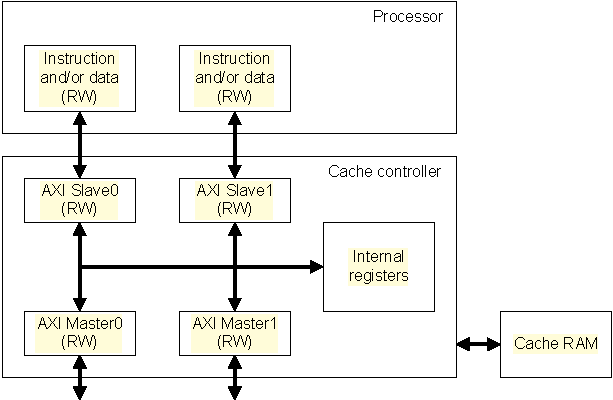
\includegraphics[width=0.9\linewidth]{example_cache_controller_interfaced_to_an_ARM_processor}
            \caption{Exemple de contrôleur de cache interfacé avec un processeur ARM \cite{manuel:coreLink_level_2_cache_controller_L2C_310}}
            \label{fig:example_cache_controller_interfaced_to_an_ARM_processor}
        \end{figure}

        \subsubsection{Impact sur les interférences}

            %\ijulien{Le cache de deuxième niveau est par défaut partagé entre les quatre cœurs du processeur peut être à l'origine de deux types d'interférences. Des \emph{interférences spatiales} lorsque les blocs de données chargés par un processeur sont évincées hors du cache par les pages utilisées par un autre cœur et des \emph{interférences temporelles} lorsque le cache reçoit un nombre de requêtes supérieur à celui qu'il peut gérer en parallèle, le premier type d'interférence pouvant être éliminé en utilisant le mécanisme matériel de verrouillage.}

            Le cache de deuxième niveau étant partagé entre les quatre cœurs du processeur, il est un canal pour deux types d'interférences.

            Tout d'abord, les caches partagés sont un canal d'interférence spatiale.
            Une application ordonnancée sur un cœur peut en effet évincer à son profit les données d'un applicatif ordonnancé sur un autre cœur.
            Il s'agit d'une des interférences le plus souvent mises en avant dans la littérature.
            Elles peuvent néanmoins être prévenues avec de la coloration de pages ou de manière équivalente avec la fonctionnalité de \emph{lockdown by master} fournie par notre carte.

            Le deuxième type d'interférences est temporel et à lieu au niveau du contrôleur PL310.
            En effet, ce dernier peut traiter un certain nombre de requête en parallèle.
            Lorsque sa capacité de traitement est dépassée, les requêtes sont traitées séquentiellement.
            Une politique d'arbitrage doit alors être appliquée sur les requêtes à traiter.
            Or, cette dernière n'est malheureusement pas documentée.

            % Si la présence de compteurs matériels au sein du cache L2, permet d'obtenir une mesure globale du trafic mémoire qui est généré par l'ensemble des cœurs, elle ne permet pas de différencier les différents cœurs consommateurs. Or, nous avons vu dans la section \ref{processeur:impacts_sur_nos_travaux} que les compteurs locaux à chaque cœur ne permettaient pas de mesurer la consommation effectuée dans les niveaux partagés de la hiérarchie mémoire. La mise en place d'une solution de régulation similaire à celle utilisée par MemGuard décrite précédemment dans la partie \ref{subsubsection:memguard} est donc impossible sur notre plate-forme.

    \subsection{Contrôleur mémoire}
    \label{subsection:controleur_memoire}

        %\itodo{Figure supprimer les bus inutilisés}

        \begin{figure}[!ht]
            \centering
            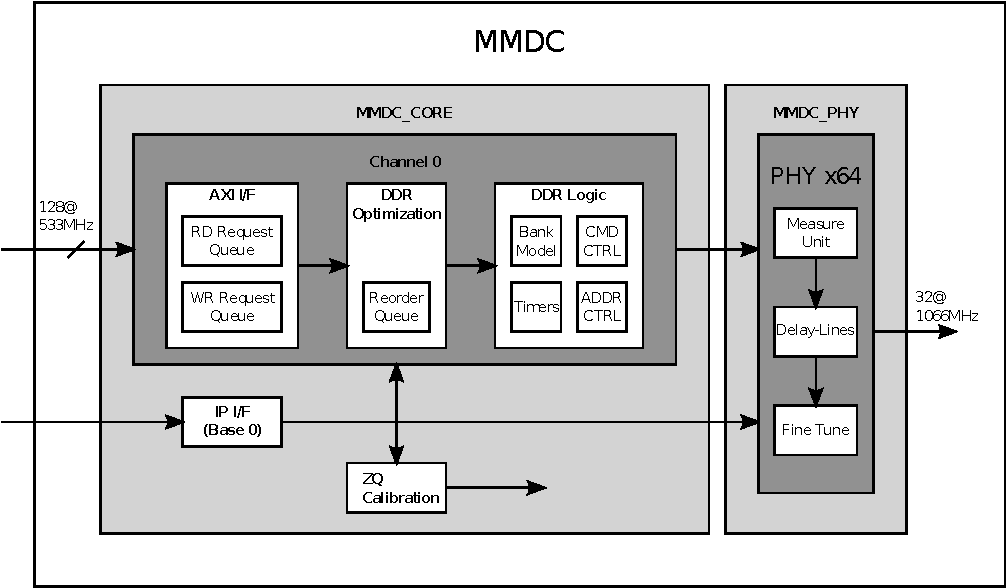
\includegraphics[width=\linewidth]{mmdc_block_diagram_2}
            \caption{Diagramme de bloc du contrôleur MMDC  \cite{manuel:i_MX_6Dual_6Quad_applications_processor_reference_manual}}
            \label{fig:mmdc_block_diagram_2}
        \end{figure}

        Le contrôleur mémoire MMDC (\emph{Multi Mode DDR Controller}) conçu par Freescale est chargé de gérer la mémoire DRAM de la plateforme matérielle. Il est constitué de deux composants, le \emph{cœur}, connecté à l'interconnecte NIC-301 par un bus AXI, gère la génération et l'optimisation des \emph{commandes mémoire} tandis que la partie \emph{PHY}, connectée à 1 giga de mémoire de type DDR3 \cite{manuel:SABRE_lite_hardware_user_manual} par un seul canal, est responsable de la gestion des \emph{timings}.

        %The MMDC module is a DDR controller that can support several types of DDR memories and two channel x32 and x64 memory widths.
        %MMDC is a multi-mode DDR controller that supports DDR3/DDR3L x16/x32/x64 and LPDDR2 two channel x16/x32 memory types. MMDC is configurable, high performance, and optimized.

        %MMDC consists of a core (MMDC\_CORE) and PHY (MMDC\_PHY).
        %\begin{itemize}
        %    \item The core is responsible for communication with the system through an AXI interface, DDR command generation, DDR command optimizations, and a read/write data path.
        %    \item The PHY is responsible for the timing adjustment; it uses special calibration mechanisms to ensure data capture margin at a clock rate of up to 533 MHz.
        %\end{itemize}

        %The core is composed of two channels, but both channels are only active in LPDDR2 mode. If DDR3 mode is selected, channel1 is not activated and the MMDC communicates with the system through AXI port0.

        Le cœur du contrôleur contient deux tampons \emph{FIFO} utilisés pour stocker temporairement les requêtes d'accès mémoire émises par les consommateurs. Le premier tampon est capable de sauvegarder jusqu'à 8 requêtes d'accès en écriture tandis que le deuxième, qui dispose d'une capacité de 16 entrées, est utilisé pour sauvegarder les requêtes d'accès en lecture.
        %
        Un mécanisme d'arbitrage de type \emph{round-robin} est utilisé pour sélectionner les requêtes d'accès en lecture et en écriture qui sont en attente et les envoyer dans un tampon intermédiaire de réordonnancement.

        Un mécanisme d'arbitrage est utilisé pour élire une requête au sein du tampon de réordonnancement et l'envoyer vers l'étage \emph{DDR Logic}, qui le découpe en commandes mémoire transmises à la mémoire DDR à travers le composant PHY. Une fois que les accès à la mémoire sont finis, la requête élue est supprimée du tampon de réordonnancement.
        %
        Le contrôleur mémoire met en œuvre une politique de gestion des \emph{row-buffer} de type \emph{open-row} que nous avons précédemment décrite en section \ref{subsection:controleur_memoire}.
        %
        %\optionnel{Le décodage d'adresse utilisé par le contrôleur mémoire est configurable. Il est notamment possible de choisir la politique de placement des données au sein des bancs mémoires. La politique de rafraîchissement du contrôleur mémoire est également configurable.}
        %
        Le décodage d'adresses utilise une politique de \emph{bank interleaving} dans laquelle les lignes consécutives en mémoire sont placées dans des bancs consécutifs.
        
        Afin d'optimiser l'utilisation du bus DDR, les requêtes d'accès sont réordonnancées dans le tampon de réordonnancement.
        Les requêtes présentes dans le tampon se voient attribuer un score afin de déterminer leur priorité, la requête avec le score le plus élevé est sélectionnée pour être envoyée vers le composant \emph{DDR logic}.
        Le score final est calculé en additionnant quatre facteurs différents et en tronquant les quatre bits de poids faibles:
        \begin{enumerate}
            \item \emph{Dynamic jump score} Ce score est incrémenté à chaque fois qu'une requête n'est pas sélectionnée.
            Ce score a une valeur maximale, égale à 15 sur notre cible.
            Lorsque cette valeur est atteinte, un mécanisme anti-famine est activé.
            
            \item \emph{Page hit score} Il s'agit d'un score statique attribué lorsque la ligne de destination de la requête est chargée dans un row buffer.
            Sur notre cible, ce score est égal à 4.
            
            \item \emph{Access score} Il s'agit d'un score statique attribué lorsque le type de l'accès (lecture ou écriture) est le même que celui de la requête sélectionnée précédemment.
            Sur notre cible, ce score est égal 2.

            \item \emph{QoS score} Il s'agit ici d'un score attribué dynamiquement par le matériel. Il est encodé sur 4 bits et ne peut donc pas dépasser 15. Mis à part cela, son mode de calcul n'est pas connu. Lorsque le mode temps réel du contrôleur mémoire est activé, toutes les requêtes avec un score QoS maximal deviennent prioritaires sur les autres requêtes.
        \end{enumerate}

        \begin{figure}[!h]
            \centering
            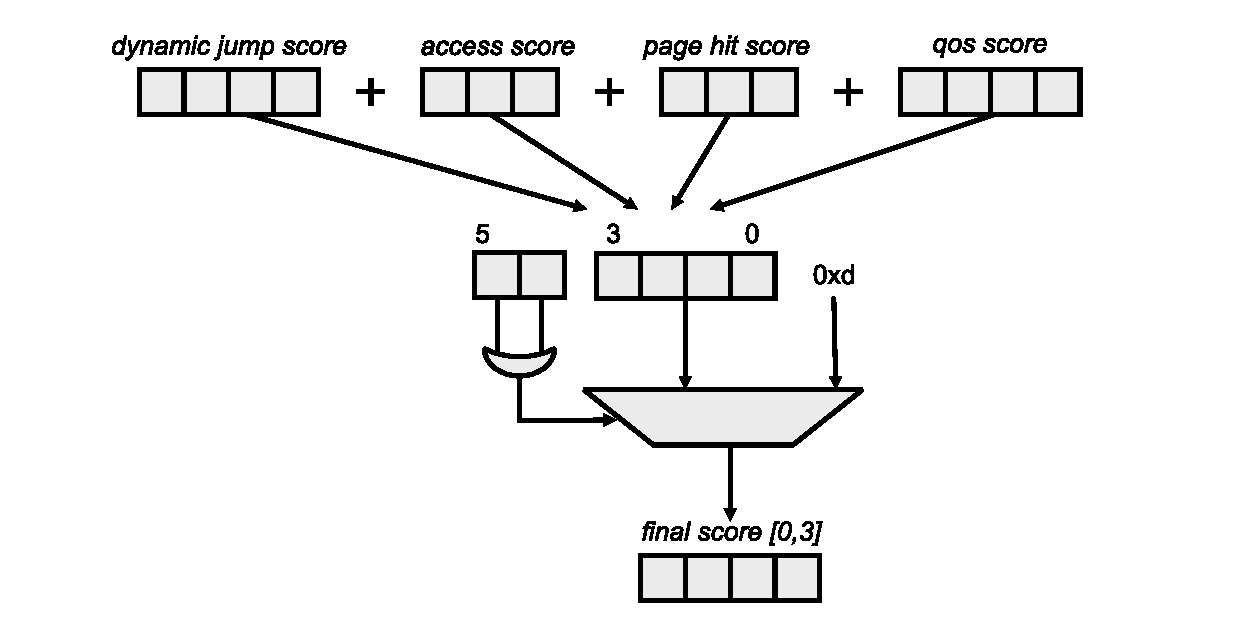
\includegraphics[width=0.75\linewidth]{mmdc-arbitration-score}
            \caption{\label{fig:mmdc_score}Calcul de la priorité lors du réordonnancement des accès DRAM}
        \end{figure}

        Lorsque le \emph{dynamic jump score} d'un accès atteint la valeur maximale, un mécanisme anti-famine est activé: un second compteur est incrémenté, jusqu'à atteindre une valeur maximale (fixée à 15 sur notre plateforme). 
        Lorsque le compteur associé à une requête atteint une valeur maximale, cette requête prend la priorité sur toutes les autres.

        Pour augmenter les performances de la mémoire, un mécanisme désactivable de prédiction permet de prédire, en parallèle du mécanisme d'arbitrage, la puce, le banc mémoire et la ligne qui vont être utilisée afin de préparer en avance la gestion des futurs accès. Selon la documentation~\cite{mmdc_dbi}, la prédiction se fait en utilisant notamment en considérant les accès au niveau du processeur, et du tampon de réordonnancement.

        Le contrôleur mémoire dispose d'un dispositif de profilage permettant de récupérer des statistiques sur l'utilisation de la mémoire (nombre d'accès effectués en lecture/écriture, trafic mémoire généré en lecture/écriture) et sur l'occupation du contrôleur mémoire (Nombre de cycles où le contrôleur est occupé). Un mécanisme de filtrage utilisant l'identifiant des bus AXI peut être mis en place pour éviter de comptabiliser le trafic mémoire généré par certains composants matériels (GPU, Ethernet, ....).

        \subsubsection{Impacts sur nos travaux}

            %\ijulien{
            %Le contrôleur mémoire va collecter l'ensemble des requêtes émis par les consommateurs pour les traduire, séquentiellement, en commandes mémoire. De multiples sources d'interférences sont présentes au sein de ce composant matériel.

            %Tout d'abord le nombre de requêtes pouvant être mises en attente au sein du contrôleur est borné, des requêtes devant être émises lorsque les tampons sont pleins doivent être retardée.

            %Ensuite, le contrôleur met en œuvre un algorithme sophistiqué qui à pour objectif d'augmenter le débit mémoire total de la plate-forme matérielle sans accorder une importance particulière aux performances temps réel de la machine. Les requêtes mémoires peuvent donc être réordonnancée, un processus effectuant une suite de commandes d'un même type (lecture ou écriture) vers une même \emph{row-buffer} se voyant priorisé par rapport à des processus effectuant un mixte de lecture et d'écritures.

            %L'utilisation d'une politique de \emph{bank interleaving} permet légalement d'accroître les performances au détriment de la prédictibilité, les données accédées par un processus se voyant réparties sur plusieurs bancs mémoire utilisés également par d'autres consommateurs.

            %Si la présence d'un mode temps réel au sein du contrôleur mémoire est prometteur puisqu'il permet de rajouter de la prédictibilité au détriment des performances, il ne peut être utilisé à la granularité d'un cœur, ce qui ne correspond pas à nos besoins.}

            %\itodo{Problème dans la partie d'avant je ne dis pas que le tag QoS est pas applicable}

            De multiples sources d'interférences sont présentes au sein du contrôleur mémoire qui va collecter l'ensemble des requêtes émises par les consommateurs pour les traduire, séquentiellement, en commandes mémoire.

            Tout d'abord, le nombre de requêtes pouvant être mises en attente au sein du contrôleur est borné par la taille des tampons de stockage des requêtes. Un consommateur qui émet un grand nombre de requêtes mémoires peut donc remplir les tampons du contrôleur retardant ainsi le traitement des requêtes des autres demandeurs.

            Une autre source d'interférences réside dans le réordonnancement des requêtes d'accès.
            En effet, le contrôleur cherche à maximiser les performances globales de la machine tout en évitant les conflits entre requêtes.
            Pour y arriver, le contrôleur mémoire réordonnance les requêtes de telle sorte à maximiser le débit mémoire total de la plateforme matérielle sans accorder une importance particulière aux performances temps réel de la machine. Un processus effectuant une suite de commandes de même type (lecture ou écriture) vers un même \emph{row-buffer} se voyant priorisé par rapport à des processus effectuant une combinaison de lectures et d'écritures.
            %
            Par conséquent, un programme qui effectue des accès favorisant une bonne bande passante peut devenir prioritaire et retarder les accès effectués par un autre programme exécuté en parallèle.

            L'utilisation d'une politique de \emph{bank interleaving} permet également d'accroître les performances au détriment de la prédictibilité, les données accédées par un processus se voyant réparties sur plusieurs bancs mémoire utilisés également par d'autres consommateurs.

            Enfin, l'utilisation d'une politique de gestion des pages de type \emph{open-row}, telle qu'utilisée par le contrôleur MMDC, introduit des dépendances temporelles entre les commandes mémoire. En effet, les temps d'accès à une cellule mémoire sont conditionnés par l'état du banc mémoire qui dépend des commandes exécutées précédemment. Des commandes mémoire émises par un cœur critique peuvent donc entrer en conflit avec celles émises par un cœur non critique générant ainsi des ralentissements.

        % \paragraph{Functional Description}
        %
        %     \subparagraph{Write data flow}
        %
        %         \begin{enumerate}
        %             \item Write requests are received into an 8 entries request FIFO. Access is received only when there are at least two available entries. Each entry holds all of the AXI attributes.
        %             \begin{itemize}
        %                 \item If the burst length is greater than 8, the access splits into two accesses: one with burst length 8 and the other with the remainder.
        %                 \item The access can be performed as soon as the entire data phase of the associated write request is completed (all data beats were received).
        %             \end{itemize}
        %             \item  A simple round-robin arbitration between the pending read and write accesses is performed, and the pointer to this stage's winner access is sent to the re-ordering buffer.
        %             \item The reordering mechanism is activated to find the winner access, which is the access that best utilizes the DDR bus, based on its dynamic score. For further information see Dynamic scoring mode (Arbitration Winning Conditions).
        %             \item  The winner write access at the previous stage is received and is held for dispatch to the DDR logic.
        %             \item  When the DDR command control unit is ready to accept the write request, it issues (if needed) a precharge/active command to the DDR device according to the status of the bank model and the parameters of the timers.
        %             \item  The DDR logic drives the associated data to the DDR device through the DDR PHY.
        %         \end{enumerate}
        %
        %     \subparagraph{Read data flow}
        %
        %         \begin{enumerate}
        %             \item Read requests are received into a 16 entry request FIFO in MMDC if there are at least two available entries. Each entry holds all of the AXI attributes. NOTE If the burst length is greater than 8, the access splits into 2 accesses (one with burst length 8 and the other with the remainder).
        %             \item A simple round-robin arbitration between the pending read and write accesses is performed and the pointer to this phase's winner access is sent to the re-ordering buffer.
        %             \item The reordering mechanism is activated to find the winner access, which is the access that best utilizes the DDR bus, based on its dynamic score. For further information see Dynamic scoring mode (Arbitration Winning Conditions).
        %             \item The winner read access at the previous stage is sampled and is held for dispatch to the DDR logic. This read access will be dispatched when there is at least one free slot in the read data buffer to store the data.
        %             \item When the DDR command control unit is ready to accept the read request, it issues (if needed) a precharge/active command to the DDR device according to the status of the bank model and the parameters of the timers.
        %             \item The MMDC PHY samples the read data, and the DDR logic transfers the data to the associated slot in the read data buffer.
        %             \item MMDC transfers the data back to the master.
        %         \end{enumerate}

        % \subparagraph{Address decoding}
        %
        %     The following registers in the MMDC define the DDR address space:
        %     \begin{itemize}
        %         \item MDMISC[DDR\_4\_BANK]—Defines either 4 or 8 banks in the DDR device
        %         \item MDCTL[DSIZ]—Defines the DDR data bus width of x16, x32 or x64
        %         \item MDMISC[BI]—Defines whether bank interleaving is on or off
        %         \item MDCTL[COL]—Defines the column size of the DDR device
        %         \item MDCTL[ROW]—Defines the row size of the DDR device
        %     \end{itemize}

        % \subparagraph{Chip select settings}
        %
        %     MMDC drives the incoming access to either CS0 or CS1 by comparing the 7 most significant address bits (ARADDR[31:25]/AWADDR[31:25]) with MDASP[CS0\_END].

        % \subparagraph{Refresh Scheme}
        %
        %     The periodic auto refresh can be triggered by the following clocks:
        %     \begin{itemize}
        %         \item 32KHz clock
        %         \item 64KHz clock
        %         \item MMDC operating clock
        %     \end{itemize}

        % \subparagraph{Burst Length options towards DDR}
        %
        % The MMDC supports two kinds of burst lengths which can be configured through MDCTL[BL] as follows: In DDR3 mode, only burst length 8 can be used.
        %
        % In DDR3 mode read/write accesses to the DDR are always 8 words (x16, x32, x64) and aligned in according to JEDEC standards.


        % \paragraph{Performance}

        % \subparagraph{Arbitration General}
        %
        %     The following specifies arbitration and reordering flow in MMDC towards the DDR.
        %     \begin{itemize}
        %         \item AXI read and write accesses are sampled in the associated queue.
        %         \item Read/write arbitration is handled to select the winning access.
        %         \item Winning access is sampled in the reordering queue
        %         \item Reordering mechanism is handled between valid requests that reside in the reordering queue to select the access that will be dispatched to the DDR.
        %         \begin{itemize}
        %             \item The reordering is held in order to optimize the accesses and to maximize the utilization of the DDR bus
        %             \item As soon as the reordered access is completed (indicated by end of response or data phase) then it is erased from the associated queue and the MMDC is ready to receive the next available access from the master
        %         \end{itemize}
        %     \end{itemize}
        %
        %     In general, the reordering/arbitration mechanism is based on dynamic priority mechanism, which compares dynamic priorities between valid entries in the reordering queue and issues the entry with highest dynamic priority towards the DDR Logic.
        %
        %     The selection of the winning access is based on two modes, which can be activated together, as following:
        %     \begin{itemize}
        %         \item Real time channel mode:
        %         \item Accesses with QoS='f' (i.e. awqos[3:0]/arqos[3:0] = "f") will bypass all other requests towards the DDR
        %         \item Dynamic scoring mode:
        %         \item The arbitration mechanism is based on dynamic priority. Relevant for the accesses with QoS smaller than 'f' or when real time channel mode is disabled.
        %     \end{itemize}
        %
        %     Due to re-ordering and optimization mechanism (per different AXI ID), the transactions towards the DDR may be driven in a different ID order they were received by the AXI master. In similar way, the write response, read response or read data may be driven to the AXI master in a different ID order.
        %
        % \subparagraph{Real time channel mode}
        %
        %     When real time mode is enabled (i.e MAARCR[ARCR\_RCH\_EN] = "1") , all requests with QoS='f' (i.e. awqos[3:0]/aqqos[3:0] = "f") will bypass all other pending accesses towards the DDR. This mode is enabled by default.
        %
        % \subparagraph{Dynamic scoring mode (Arbitration Winning Conditions)}
        %
        %     The arbitration between pending accesses in the MMDC is handled according to a dynamic priority of each access.
        %
        %     The dynamic priority (may be also called score) is calculated according to a sum of some factors (final\_score[3:0]), where part of them may be updated dynamically. The following will specify each scoring factor:
        %
        %     \begin{itemize}
        %         \item MAARCR[ARCR\_PAG\_HIT] (Page hit score) - A static score which is taken into account in case the pending access has a page hit
        %         \item MAARCR[ARCR\_ACC\_HIT] (Access hit score) - A static score, which is taken into account in case the current access type (read/write) is the same as the access that has been dispatched to the DDR previously
        %         \item MAARCR[ARCR\_DYN\_JMP] (Dynamic jump score) - A dynamic score which is given to any pending access in case it was not chosen in the arbitration. The dynamic jump counter is limited by maximum value which is set in MAARCR[ARCR\_DYN\_MAX] .
        %         \item QoS score which is indicated through a sideband 4bits AXI signals (awqos[3:0]/aqqos[3:0]) and is driven by the AXI master per access
        %     \end{itemize}
        %
        %     Note: In order to prevent an overflow in the total sum of scores, a clipping is held and selects the maximum score value of 'f' once a total scores sum is greater than 'f'.
        %
        % \subparagraph{Guarding (aging) mechanism}
        %
        %     The guarding mechanism (may be also called aging) is used to prevent a starvation of accesses.
        %
        %     As soon as the dynamic jump score reaches its maximum value (MAARCR[ARCR\_DYN\_MAX] ) then each time a pending request was not chosen in the arbitration, the "guarding" counter is incremented by 1. When the "guarding" counter reaches its predefined value, set in MAARCR[ARCR\_GUARD], the associated request gets the highest priority and will be chosen in the next arbitration cycle towards the DDR unless a real time channel (i.e access with QoS ="f") is arrived.
        %
        %     Note: In case real time channel has arrived then the dynamic score of the non real time channels won't increment in order to prevent a case where the "guarding" counter of more than one access has reached its limit.

        % \subparagraph{Prediction mechanism}
        %
        %     When prediction mechanism is enabled (i.e by configuring MDMISC[MIF3\_MODE]) then the MMDC predicts the chip-select, bank address and row address that is going to be issued towards the DDR before the access is physically dispatched towards DDR device. That mechanism enables to prepare the DDR device with future accesses and improves the overall DDR performance.
        %
        %     This prediction mechanism operates in parallel to the reordering mechanism and may yield a prediction based on 3 levels of pending accesses:
        %     \begin{enumerate}
        %         \item Access in first stage of pipeline.
        %         \item Valid access on AXI bus either read channel or write channel.
        %         \item Valid access on special bus from arbit
        %     \end{enumerate}

%             \paragraph{MMDC Profiling}

        % The profiling mechanism provides the ability to calculate the DDR utilization together with read and write accesses statistics towards DDR per given period of time.
        %
        % MMDC supports the following profiling counters:
        % \begin{itemize}
        %     \item MADPSR0 (Total cycles count) - Indicates the total amount of cycles of the profiling period (up to 2^32 cycles)
        %     \item MADPSR1 (Busy cycles count) - Indicates the total busy cycles during the profiling period
        %     \item MADPSR2 (Total read accesses count) - Indicates the total read accesses towards MMDC during the profiling period
        %     \item MADPSR3 (Total write accesses count) - Indicates the total write accesses towards MMDC during the profiling period
        %     \item MADPSR4 (Total read bytes count) - Indicates total bytes that were read from MMDC during the profiling period
        %     \item MADPSR5 (Total write bytes count) - Indicates total bytes that were written to MMDC during the profiling period
        % \end{itemize}
        %
        % Read/Write statistics can be collected per specific AXI ID (16bits). The following fields in MADPCR1 register determines which AXI-ID or AXI-ID's to monitor:
        % \begin{itemize}
        %     \item PRF_AXI_ID defines which AXI IDs are taken for profiling. Default values is 16'h0.
        %     \item PRF_AXI_ID_MASK defines which bits from PRF_AXI_ID will be compared with AXI ID of read/write access. "1" means to monitor the associated bit and "0" means don't care. Default value is 16'h0000, meaning all IDs are monitored
        % \end{itemize}

        % Table 6-1. MMDC feature summary
        %
        % Supported standards • LV-DDR3, DDR3 x16, x32, x64 (includes SODIMM)
        %     • LPDDR2 2ch x32, in either split map or interleaving mode
        %     • LPDDR2 1ch x32
        %
        % DDR interface • x16, x32, x64 data bus width
        %     • Density of 256 Mbytes-8 Gbytes
        %     • Column size of 8-12 bits
        %     • Row size of 11-16 bits
        %     • 2 CS per channel, with a separate CS allocation for LPDDR2-DRAM)
        %     • Up to 4 Gbyte address space and configurable address space per CS. For LPDDR2 2ch x32 up to 2 Gbytes per channel
        %     • Interleaved accesses of LPDDR2-DRAM towards the same DDR channel. This is supported only when using the same clock frequency for LPDDR2-DRAM
        %     • Supports burst length of 8 (aligned) for DDR3 and burst lengths of 4 for LPDDR2
        %
        % DDR performance
        %     • DDR3 and LPDDR2 support up to 1066MT/s transfer rate
        %     • Supports Real-Time priority by means of QoS sideband priority signals from the chip to enable different priority levels in the re-ordering mechanism
        %     • Page hit/page miss optimizations
        %     • Consecutive read/write access optimizations
        %     • Supports deep read and write requests queues to enable bank prediction
        %     • Drives back the critical word in a read transaction as soon as it is received by the DDR device (doesn't wait until the whole data phase has been completed)
        %     • Can track open memory pages
        %     • Supports bank interleaving
        %     • Special optimization for non-aligned wrap accesses in burst length 8 AXI interface
        %     • AXI bus compliant with glueless interface to PL301 AXI network interconnect
        %     • Supports bus transfers of 8,16,32, 64 and 128 bits (single accesses and bursts)
        %
        % DDR calibration and delay-lines
        %     • All calibrations can be done automatically by hardware or manually by software
        %     • ZQ calibration for external DDR device (in DDR3 through the ZQ calibration command and in LPDDR2 through the MRW command).
        %     • Can be handled automatically for ZQ Short (periodically) and ZQ Long (at exit from self-refresh).
        %     • Can be handled manually at ZQ INIT.
        %
        % DDR general
        %     • Configurable timing parameters
        %     • Configurable refresh scheme
        %     • Supports dynamic voltage, frequency change and low power mode entry through hardware negotiation with the system (req/ack handshake)
        %     • Suppors automatic self-refresh and power down entry and exit
        %     • Supports fast and slow precharge power down in DDR3
        %     • Supports various ODT control schemes.
        %     • Assertion/Deassertion of ODT control per read or write accesses and for active or passive CS
        %     • Supports MRW and MRR commands for LPDDR2.
        %     • Software control for moving to derated timing parameters and derated refresh rate according to temperature variation.
        %     • Supports various debug and profiling modes

    % ===============================
    % ============ netys ============
    % ===============================
    %
    %\subsection{Hardware}
    %
    %    We focus on embedded systems, as used in the automotive domain, which has strong hardware cost requirements. Therefore, for our tests we use the SABRE Lite board \cite{MANUAL:IMX6_DQRM}, a low-cost development platform designed for multimedia applications on the Android and Linux operating systems. A variant of this platform that has been adapted for the automotive domain is used by a large number of automotive manufacturers and suppliers
    %
    %    The processor of the SABRE Lite is an i.MX 6, which is based on a 1.2 GHz quad-core Cortex A9 MPCore \cite{MANUAL:A9_MPCORE_TRM}. Each core has a separate Level 1 (L1) 32-kilobyte 4-way set-associative cache for instructions and data \cite{MANUAL:A9_TRM}. All CPUs are connected to a single 1-megabyte 16-way set-associative L2 cache \cite{MANUAL:L2C310_TRM} that can be partitioned into multiples of the way size. Finally, the Multi Mode DRAM Controller (MMDC) manages access to one gigabyte of DDR3 RAM that can be used by all the cores \cite{MANUAL:IMX6_DQRM}.
    %
    %    The SABRE Lite board provides various hardware performance counters. Each core provides six configurable counters to gather statistics about the operation of the processor (number of cycles) and the memory system (L1 cache hits/misses) \cite{MANUAL:ARMV7,MANUAL:A9_TRM}. The MMDC has a profiling mechanism that gathers statistics (read/write bytes/access)  about the global memory traffic on the platform.

    % ===============================
    % ============ ECRTS ============
    % ===============================
    %
    %\subsection{Architecture of the SABRE Lite}

    %    In this paper, we target embedded systems, as used in the automotive domain, which has strong hardware cost requirements. We choose the SABRE Lite multicore system \cite{MANUAL:IMX6_DQRM} (see Figure~\ref{fig:archiIMX6}) since it has already been adopted by some industry leaders as an experimental platform.

    %    The processor of the SABRE Lite is an i.MX 6, which is based on a 1.2 GHz quad-core Cortex A9 MPCore \cite{MANUAL:A9_MPCORE_TRM}. Each core has two 32-kilobyte 4-way set-associative L1 caches, one for data and the other for instructions. Each core is also connected to an external 1-megabyte 16-way set-associative L2 cache \cite{MANUAL:L2C310_TRM} that can be either shared by all the cores or partitioned in multiples of 1/16th of the cache size. The Multi Mode DRAM Controller (MMDC) manages access to one gigabyte of DDR3 RAM that can be used by all cores \cite{MANUAL:IMX6_DQRM}. Each core contains six configurable hardware counters to gather statistics on the operation of the processor (number of cycles, etc.) and the memory system (L1 accesses, L1 misses, etc.) \cite{MANUAL:ARMV7, MANUAL:A9_TRM}.  The MMDC contains hardware counters that measure global memory traffic (read/write bytes, read/write accesses, etc.)  on the platform \cite{MANUAL:IMX6_DQRM}, but no hardware counter is provided to identify the core that is the source of a L2 miss.

    %    On the SABRE Lite, when using DDR3 RAM, the MMDC is accessible through a single AXI channel.  This AXI channel has two dedicated request queues: a 16 entry queue for read requests and a 8 entry queue for write requests. Each request queue entry holds the information to access up to one cache line. A round-robin arbitration mechanism is used to send pending read and write requests into a final reordering buffer, before the request is sent to the RAM.  We will show in Figure \ref{microbench_delay_bandwidth} that this mechanism has a significant impact on the bandwidth that can be achieved when mixing read and write accesses.

        % \begin{figure}[!ht]
        %     \centering
        %     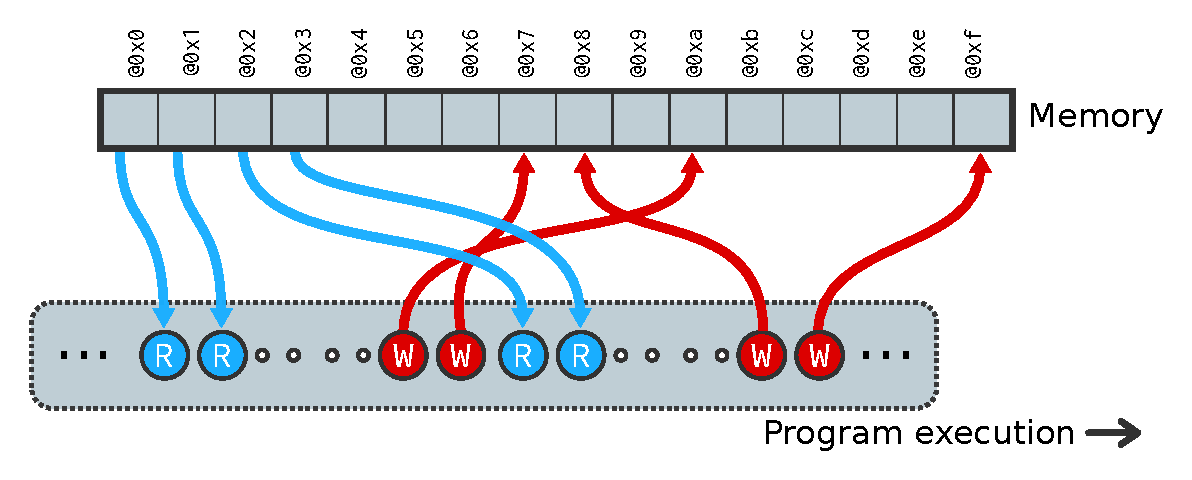
\includegraphics[scale=0.4]{memory}
        %     \caption{Architecture of the SABRE Lite board}
        %     \label{fig:archiIMX6}
        % \end{figure}

    %\subsection{Autre}
    %
    %    \itodo{Faut-il détailler les TLBs?}
    %    \ijulien{Oui mais pas le temps}
    \subsection{Récapitulatif}

Le tableau \ref{table:recapitulatif_hierarchie_memoire} contient, pour les multiples niveaux de la hiérarchie mémoire de notre carte, un récapitulatif des différentes caractéristiques matérielles qui sont partie prenante du problème de contention mémoire, à savoir, la taille et la politique de correspondance et de remplacement des différents composants.
        %
Dans une dernière colonne, nous avons aussi noté les métriques disponibles pour l’élaboration d’un nouveau mécanisme de contrôle.

\begin{table}[!h]
    \renewcommand{\arraystretch}{1.5}
    \resizebox{\linewidth}{!}{
    \begin{tabular}{l l l l l l}
        \toprule
        \multicolumn{2}{l}{\textbf{}} & \textbf{} & \textbf{} & \textbf{} & \textbf{Métriques}\\
        \multicolumn{2}{l}{\textbf{Composant}} & \textbf{Taille} & \textbf{Correspondance} & \textbf{Remplacement} & \textbf{Disponibles}\\
        \midrule
        \multirow{2}{*}{Cache L1} & Donnée & \multirow{2}{*}{32KiB} & 4 & PLRU ou PR & \multirow{2}{*}{PMU locale}\\
                                  & Instructions & & 4 & PR & \\
 
        \multicolumn{2}{l}{Cache L2} & 1MiB & 16 & PLRU ou PR & PMU globale \\

        \midrule
        \multicolumn{2}{l}{\textbf{}} & \textbf{} & \textbf{Nombre de bancs} & \textbf{} & \textbf{}\\
        \midrule
        \multicolumn{2}{l}{Mémoire principale} & 1GiB & 8 & N/A & PMU globale \\
        \bottomrule
        
    \end{tabular}
    }
    \caption{Récapitulatif des caractéristiques matérielles des différents niveaux de la hiérarchie mémoire.}
	\label{table:recapitulatif_hierarchie_memoire}
\end{table}
